\newcommand{\bW}{\mathbf{W}}
\newcommand{\by}{\mathbf{y}}
\newcommand{\bx}{\mathbf{x}}
\newcommand{\be}{\mathbf{e}}
\newcommand{\bD}{\mathbf{D}}
\newcommand{\te}{\tilde{\mathbf{e}}}
\newcommand{\balpha}{\boldsymbol{\alpha}}
\newcommand{\btau}{\boldsymbol{\tau}}
\newcommand{\bPhi}{\boldsymbol{\Phi}}
\newcommand{\norm}[1]{\left\|#1 \right\|}
\newcommand{\Real}{\mathbb{R}}
\newcommand{\bemx}{\begin{bmatrix}}
\newcommand{\enmx}{\end{bmatrix}}

For practical face hallucination scenarios, the input LR images might be corrupted due to occlusion or disguise, and thus it would be crucial to develop a hallucination algorithm which is robust to such undesirable effects. In our work, we propose a sparse representation based algorithm to recover the image regions of interest in the HR outputs, while the corrupted ones will be simplified predicted by interpolation based techniques (and be disregarded if recognition is performed).

Before detailing our proposed method, we first define the notations and variables for the sake of clarification. Let $\by_L\in\Real^d$ be the LR input image, which might be partially occluded. We have $\bD_L\in\Real^{d\times n}$ as the LR training dictionary of $n$ instances, i.e., $\bD_L = [\bx_{L,1},\bx_{L,2},\cdots,\bx_{L,N}]$, where $\bx_{L,i}\in\Real^d$ denotes the $i$th LR training image and $N$ is the number of training images. To solve image representation problems with occlusion, Yang \emph{et al.}~\cite{Yang_CVPR2011} recently presented robust sparse coding (RSC), which represents the LR input by solving

\begin{equation} \label{eq:RSCProblem}
\min_{\balpha_L}\norm{\bW_L(\by_L-\bD_L\balpha_L)}_2^2+\lambda\norm{\balpha_L}_1,
\end{equation}
where the weight matrix $\bW_L$ is defined as
\begin{equation}\label{eq:weight}
\begin{split}
&\bW_L = \mbox{diag}(w(e_{1}), w(e_{2}), \ldots, w(e_{d}))^{1/2},\\
&\mbox{and}~~w(e_{k}) = \frac{exp(-\mu e_{k}^{2}+\mu\delta)}{1+exp(-\mu e_{k}^{2}+\mu\delta)}.
\end{split}
\end{equation}
In~\eqref{eq:weight}, $e_k$ indicates the $k$th entry of $\mathbf{e} = \by_L-\bD_L\balpha_L$, which represents the reconstruction error for the $k$th image pixel in the LR input. The function $w(e_{k})$ is designed to produce a small value when the magnitude of $e_k$ is large (and vice versa). In~\cite{Yang_CVPR2011}, the product $\mu\delta$ is chosen to be a large constant, and $\delta$ is the $j$th largest entry in the vector $[e_{1}^{2},e_{2}^{2}\ldots e_{d}^{2}]$. RSC has $j$ as the nearest integer to $\tau d$ with $\tau \in [0.6, 0.8]$. Nevertheless, the goal of RSC is to suppress the influence of poorly reconstructed pixels.

%Note that when $\bW_L$ is fixed, \eqref{eq:RSCProblem} becomes a standard L1-minimization problem. In all of our experiments, we utilize the Homotopy method for solving \eqref{eq:RSCProblem} because of its efficiency as suggested in \cite{L1review}.

It is worth noting that $\tau$ can be interpreted as the proportion of non-occluded image pixels to the total pixel number in the LR input. For example, if we set $\tau$ as 0.6, 40\% percent of pixels associated with the largest (poorest) reconstruction errors will be suppressed. In other words, the remaining 60\% of the pixels will be recovered by $\bD_L$. Unfortunately, there is no guideline in~\cite{Yang_CVPR2011} to determine this crucial parameter $\tau$, and thus it might not be easy to apply RSC for practical scenarios.

To overcome the above problem, we propose a maximum likelihood estimation (MLE)~\cite{Bishop_2006} based approach for determine the optimal $\tau$, which allows us to recover the non-occluded image regions with performance guarantees. Instead of setting $\tau$ as a fixed value for all input images, we first observe the recovered images with varying $\tau$ values. Figure~\ref{fig_regression} shows an example, in which each point denotes the total reconstruction error for non-occluded image pixels with a particular $\tau$ value. More specifically, by varying the value of $\tau$, we obtain a set of points $(\tau_1,e_1), \ldots, (\tau_M,e_M)$.

% fig: idealCurve
\begin{figure}[!t]
\graphicspath{{fig/}}
        \begin{center}
            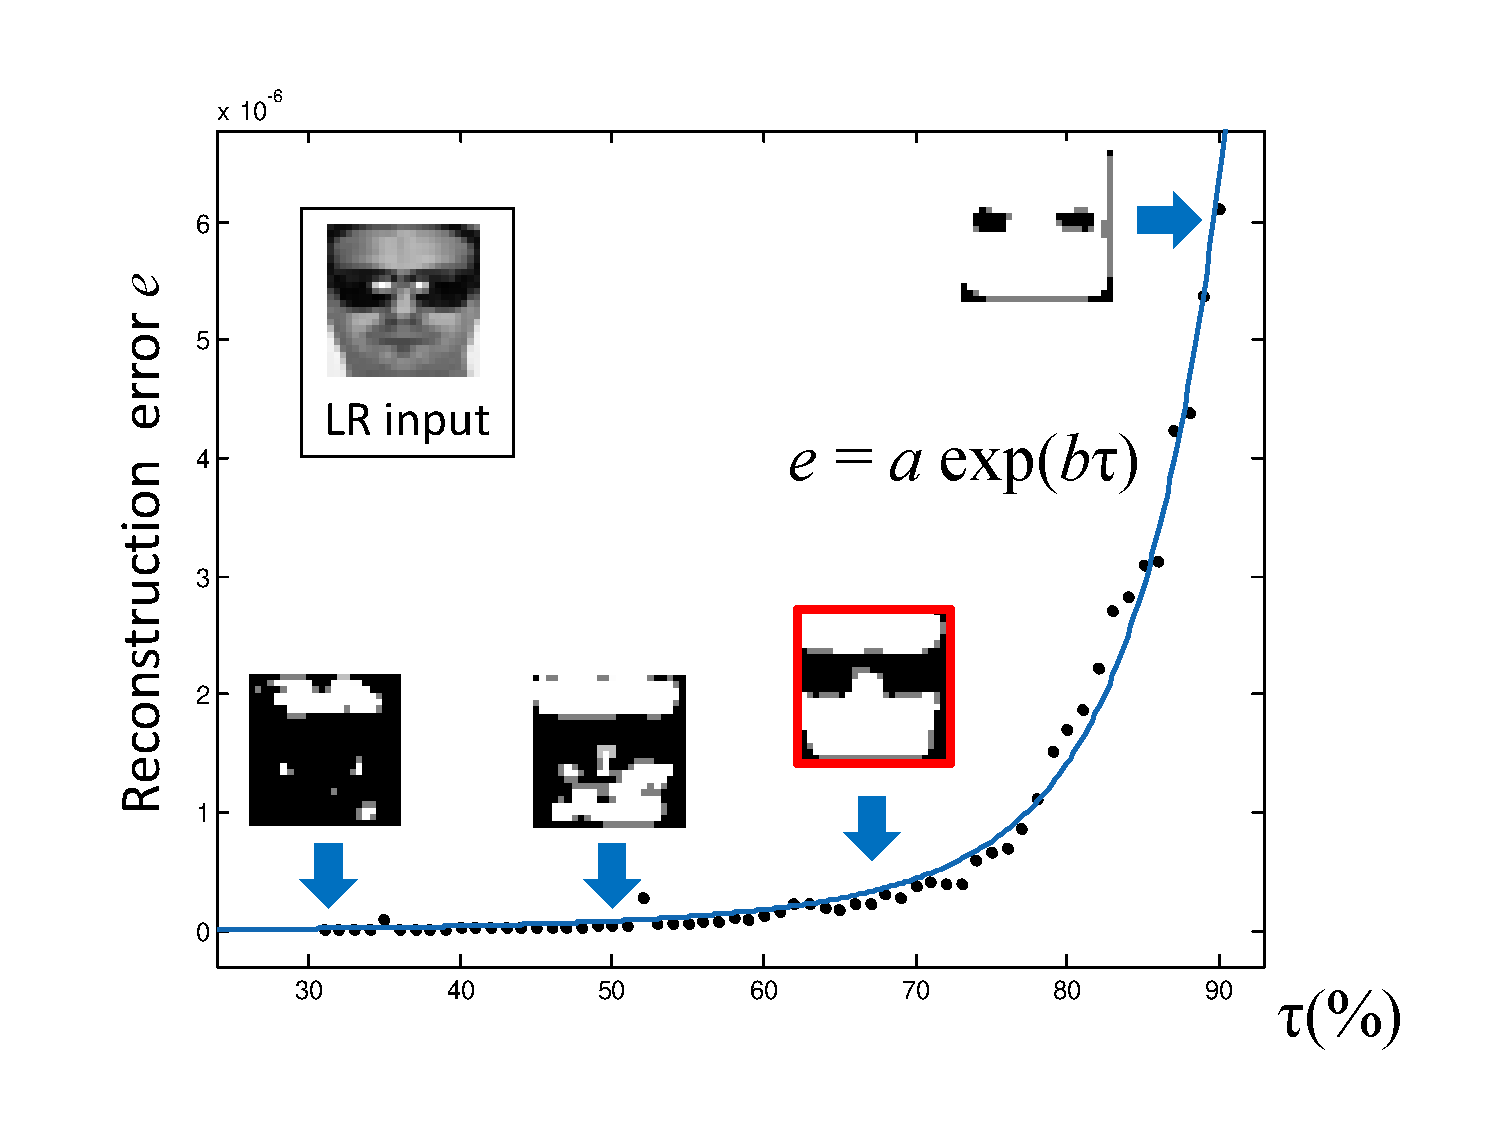
\includegraphics[scale=0.30]{exponential_regression.pdf}
            \vspace{-0.2cm}
            \caption{\small{Reconstruction errors of non-occluded image regions with varying $\tau$ values. The blue curve is an exponential function $e=a\exp(b\tau)$ fitting the observed instances. Note the the preferable recovered image is bounded by a red rectangle.}}\label{fig_regression}\vspace{-.5cm}
        \end{center}
\end{figure}

In order to determine the optimal $\tau$ for obtaining the preferable recovered face image (i.e., the one with red rectangle in Figure~\ref{fig_regression}), we need to first fit the observed points with an exponential function, i.e.,
\begin{equation}\label{eqn_exponential}
     e = f(\tau,a,b) = a\exp(b\tau),
\end{equation}
where $a$ and $b$ are the parameters to be determined. Note that $f(\tau,a,b)$ in \eqref{eqn_exponential} is a nonlinear function of $\tau$. To make the fitting problem more tractable, we take the logarithm of both sides of~\eqref{eqn_exponential} and obtain $\ln (e) = \ln (a) + b\tau$. Based on MLE, we approach this curve fitting task by solving the following optimization problem:
\begin{equation}\label{eqn_ls}
    \min_{a,b}\sum_{m=1}^M \left(\ln(e_m)-\ln(a)-b\tau_m\right)^2.
\end{equation}
By defining $\tilde{a} = \ln(a)$, the above minimization problem can be expressed as
\begin{equation}\label{eqn_ls_eq}
    \min_{\tilde{a},b} \norm{\te-[\mathbf{1}, \btau]\bemx \tilde{a}\\ b\enmx}_2^2,
\end{equation}
where $\te = [\ln(e_1),\ldots,\ln(e_M)]^T$, $\btau = [\tau_1,\ldots,\tau_M]^T$, and $\mathbf{1} = [1,\ldots,1]^T\in\Real^M$. We note that~\eqref{eqn_ls_eq} is a standard least squares problem, and its analytical solution is dervied by
\begin{equation}\label{eqn_ls_sol}
     \bemx \tilde{a}\\b \enmx = (\bPhi^T\bPhi)^{-1}\bPhi^T\te
\end{equation}
with $\bPhi := [\mathbf{1}, \btau]$. Once we have $\tilde{a}$, the parameter $a$ is obtained as $a = \exp(\tilde{a})$.

With parameters $a$ and $b$ for the exponential curve~\eqref{eqn_exponential} learned by MLE, we now discuss how to determine the optimal $\tau$ for recovering the image without occluded pixels (e.g., the one bounded by the red rectangle in Figure~\ref{fig_regression}). In our work, we empirically observe that the optimal $\tau$ always corresponds to the intersection of the reconstruction curve and the straight line with a fixed slope $s$ as shown in Figure~\ref{fig_slopes}. Moreover, this slope $s$ does \emph{not} vary with different types of face images (occluded or not).

In our work, the value of $s$ can be directly observed from training data, which is a constant over images with different degrees of occlusion (as illustrated in Figure~\ref{fig_slopes}). Once the value of $s$ is known, we can begin to calculate parameter $\tau$. To solve this task, we set the derivative of~\eqref{eqn_exponential} with respect to $\tau$ equal to $s$. As a result, we have $\frac{de}{d\tau} = ab\exp(b\tau) = s$, and the optimal $\tau$ is obtained as follows
\begin{equation}\label{eqn_tau}
     \tau = \frac{1}{b}(\ln(s)-\ln(ab)).
\end{equation}
Different from RSC which requires one to manually select $\tau$ for representing the input image, our method is able to automatically select the best $\tau$ for each input without any prior knowledge on the type of occlusion, which is preferable for practical hallucination tasks. Thus, we refer to this proposed encoding process as \emph{occlusion invariant sparse coding}.

Once the optimal $\tau$, we apply~\eqref{eq:weight} for calculating the associated weight matrix $\bW_L$. For refinement purposes, a median filter is applied to the resulting $\bW_L$ which preserves the completeness and smoothness of the determined occluded regions.




\begin{figure}
\graphicspath{{fig/}}
    \begin{center}
        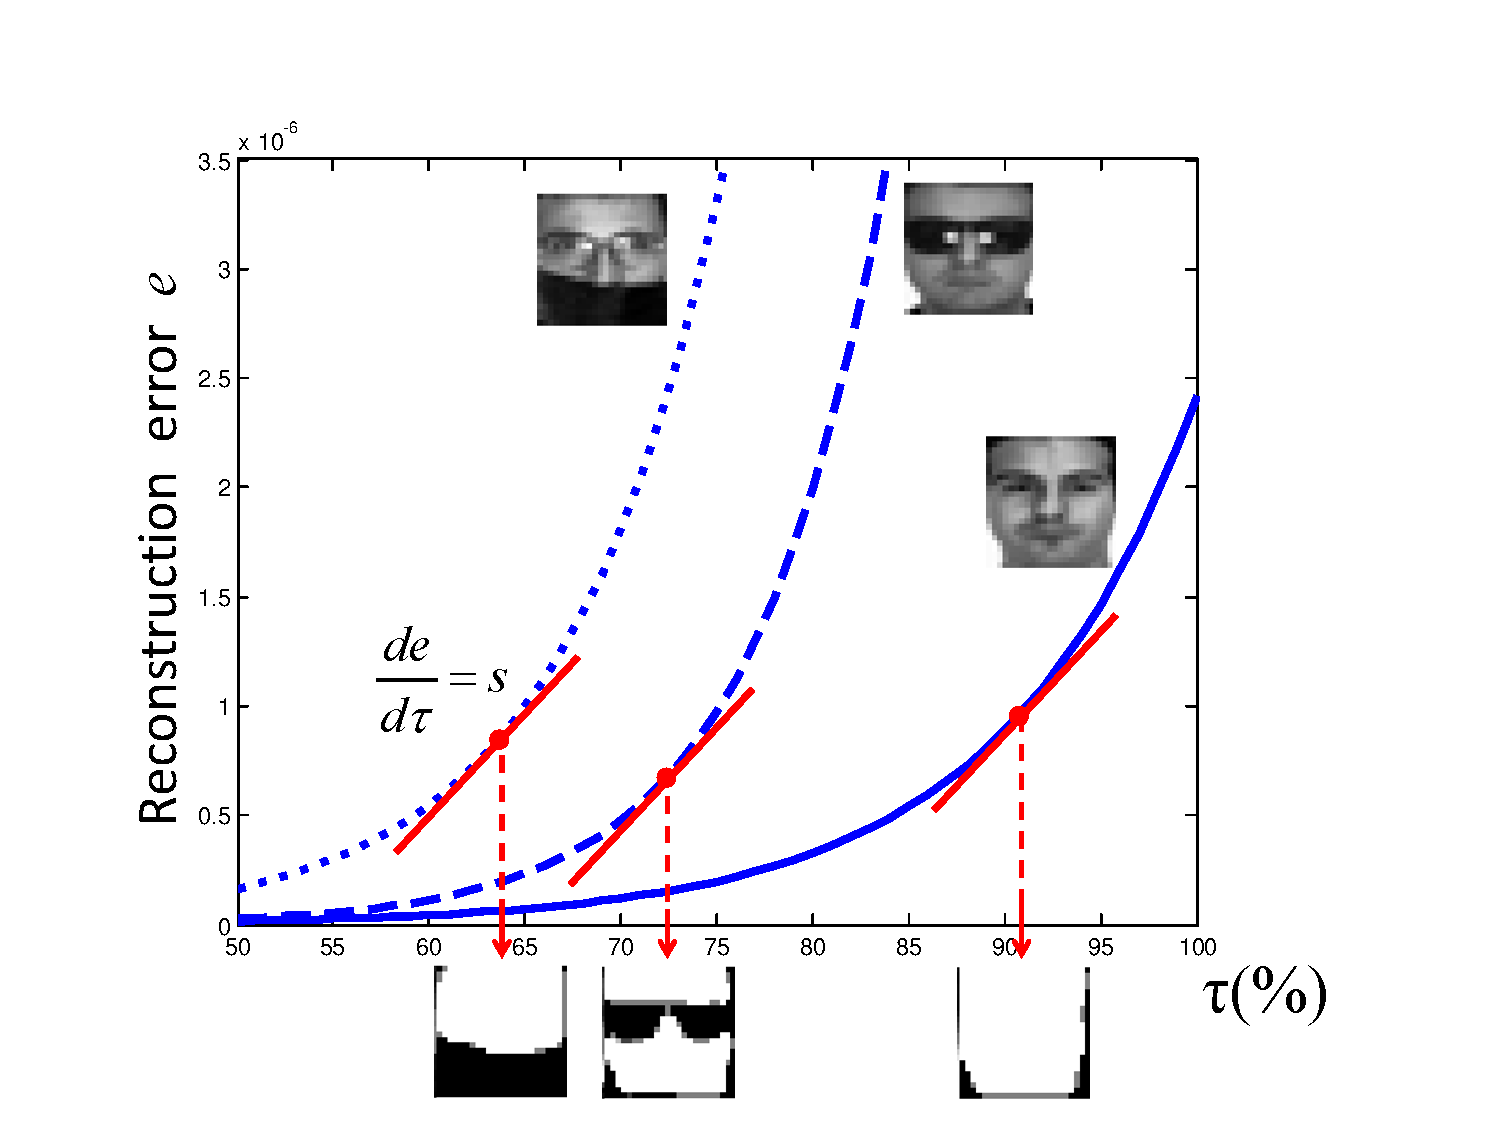
\includegraphics[scale=0.32]{ARSC_slopes.pdf}
        \vspace{-0.2cm}
        \caption{\small{Fitting curves of reconstruction errors $e$ vs. $\tau$ for three face images with different degrees of occlusion. The points of tangency depict the optimal $\tau$ for recovering non-occluded image regions.}}\label{fig_slopes}
        %\topcaption{The appropriate slope for determining $\tau$. Although the two input images (i.e., the occluded one and the neutral one) have different proportion of occluded pixels, this pre-defined slope can identify the occluded region nicely.\label{fig:cutSlope}}
    \end{center}\vspace{-.5cm}
\end{figure}
